\scanpage{109}

\begin{center}
U N I V E R S I T E\\
DES SCIENCES ET TECHNIQUES\\
DU LANGUEDOC\\
------------
\end{center}

MONTPELLIER, le 06 Octobre 1978

Service de la Scolarité\\
MR / GJ\\
Diffusion\quad : Liste H\\
N° : 5462

\begin{center}
\uline{AVIS DE SOUTENANCE D'UNE THESE DE DOCTORAT D ' ETAT}
\end{center}

\uline{Nom et prénom du candidat} : SOONCKINDT Louis

\uline{Titre de la thèse} : Contribution à l'étude des propriétés électroniques des surfaces réelles et clivées sous ultra-vide d'antimoniure de gallium.

\uline{Date, heure et lieu de soutenance prévus} : 26 OCTOBRE 1978 à 11 Heures\\
Salle de cours n° 7 - U.S.T.L.

\uline{Nom du Directeur de thèse} : Monsieur le Professeur LASSABATERE Louis.

\uline{Désignation du Laboratoire où la thèse est préparée} : C. E. E. S.

\uline{Résumé de la thèse} : Après avoir décrit le montage expérimental réalisé au Laboratoire et permettant l'étude des travaux de sortie par la méthode de Kelvin on étudie les propriétés électroniques des surfaces réelles et des surfaces propres, obtenues par clivage, de GaSb. On précise les interactions entre les états électroniques de surface (\textit{intrinsèques et extrinsèques}) dans l'obscurité et sous éclairement dans la gamme de température comprise entre 100 et $420^\circ$ K.

\uline{Durée approximative des recherches ayant abouti à la thèse} : 8 ans.

\uline{Noms des Rapporteurs} :

\diagram{$\begin{array}{lll}
\text{LASSABATERE} & \text{Louis} & \text{, Professeur, Electronique, U. S. T. L.} \\
\text{LANNOO} & \text{Maurice} & \text{Maître Recherche, Physique du Solide, ISEN LILLE} \\
\text{SEBENNE} & \text{Claude} & \text{Maître Recherche, Physique du Solide, PARIS 6}
\end{array}$}

\uline{Composition du jury proposé} :

\diagram{$\begin{array}{lll}
\text{PISTOULET} & \text{B.} & \text{Professeur, Electronique, U.S.T.L.} \\
 & & \text{Président} \\
\text{LACOSTE} & \text{R.} & \text{Professeur, Electronique, Univers. P. SABATIER, TOULOUSE} \\
\text{LANNOO} & \text{M.} & \text{Maître Recherche, Physique du Solide, ISEN LILLE} \\
\text{SEBENNE} & \text{C.} & \text{Maître Recherche, Physique du Solide, PARIS 6} \\
 & & \text{(Membre extérieur choisi en raison de sa compétence scientifique)} \\
\text{LASSABATERE} & \text{L.} & \text{Professeur, Electronique, U.S.T.L.} \\
\text{NOUGIER} & \text{J.-P.} & \text{Professeur, Electronique, U.S.T.L.} \\
 & & \text{(Membre étranger à la spécialité du candidat).}
\end{array}$}

Le Secrétaire Général,

\figure{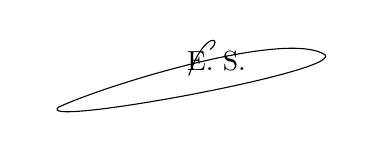
\begin{tikzpicture}[x=1cm,y=1cm]
\node at (0.7,0.33) {\unsure{E. S.}};
\draw (-1.3,-0.25) .. controls (-0.72,0.02) and (1.5,0.71) .. (2.05,0.43) .. controls (2.53,0.24) and (-1.69,-0.53) .. (-1.3,-0.25);
\draw (0.35,0.15) .. controls (0.56,0.75) and (0.8,0.62) .. (0.62,0.48);
\end{tikzpicture}}

\uline{E. S I A U}

MR LE PROFESSEUR GROTHENDIECK A.

\hfill 5

\hfill 5

MATHEMATIQUES

\mspage{108}
